\begin{frame}[t]{Input Modeling}{What the CO$_2$ input data contains}

  \begin{columns}[T,totalwidth=\textwidth]
    \begin{column}{0.48\textwidth}
      \textbf{Data from Electricity Map}
      \begin{itemize}
        \item 5 regions: DE, IT, SE, CN, US
        \item 201,600 samples per region
        \item 1,008,000 samples in total
        \item 5-minute time resolution
        \item Time span: 2022-01-01 to 2026-06-16
      \end{itemize}
    \end{column}
    \begin{column}{0.48\textwidth}
      \textbf{Data quality}
      \begin{itemize}
        \item Most values measured, not estimated.
        \item Estimated-value share below 3\% for DE, ES, SE.
        \item For China all values are estimated.
        \item Dataset is usable for region-level modeling.
      \end{itemize}
    \end{column}
  \end{columns}
\end{frame}

\begin{frame}[t]{Input Modeling}{Daily CO$_2$ intensity by region}

  \centering
  
\includegraphics[width=\textwidth,height=0.65\textheight,keepaspectratio]{assets/daily_co2_intensity.png}
\end{frame}

\begin{frame}[t]{Input Modeling}{The time series is not independent}

  \centering
  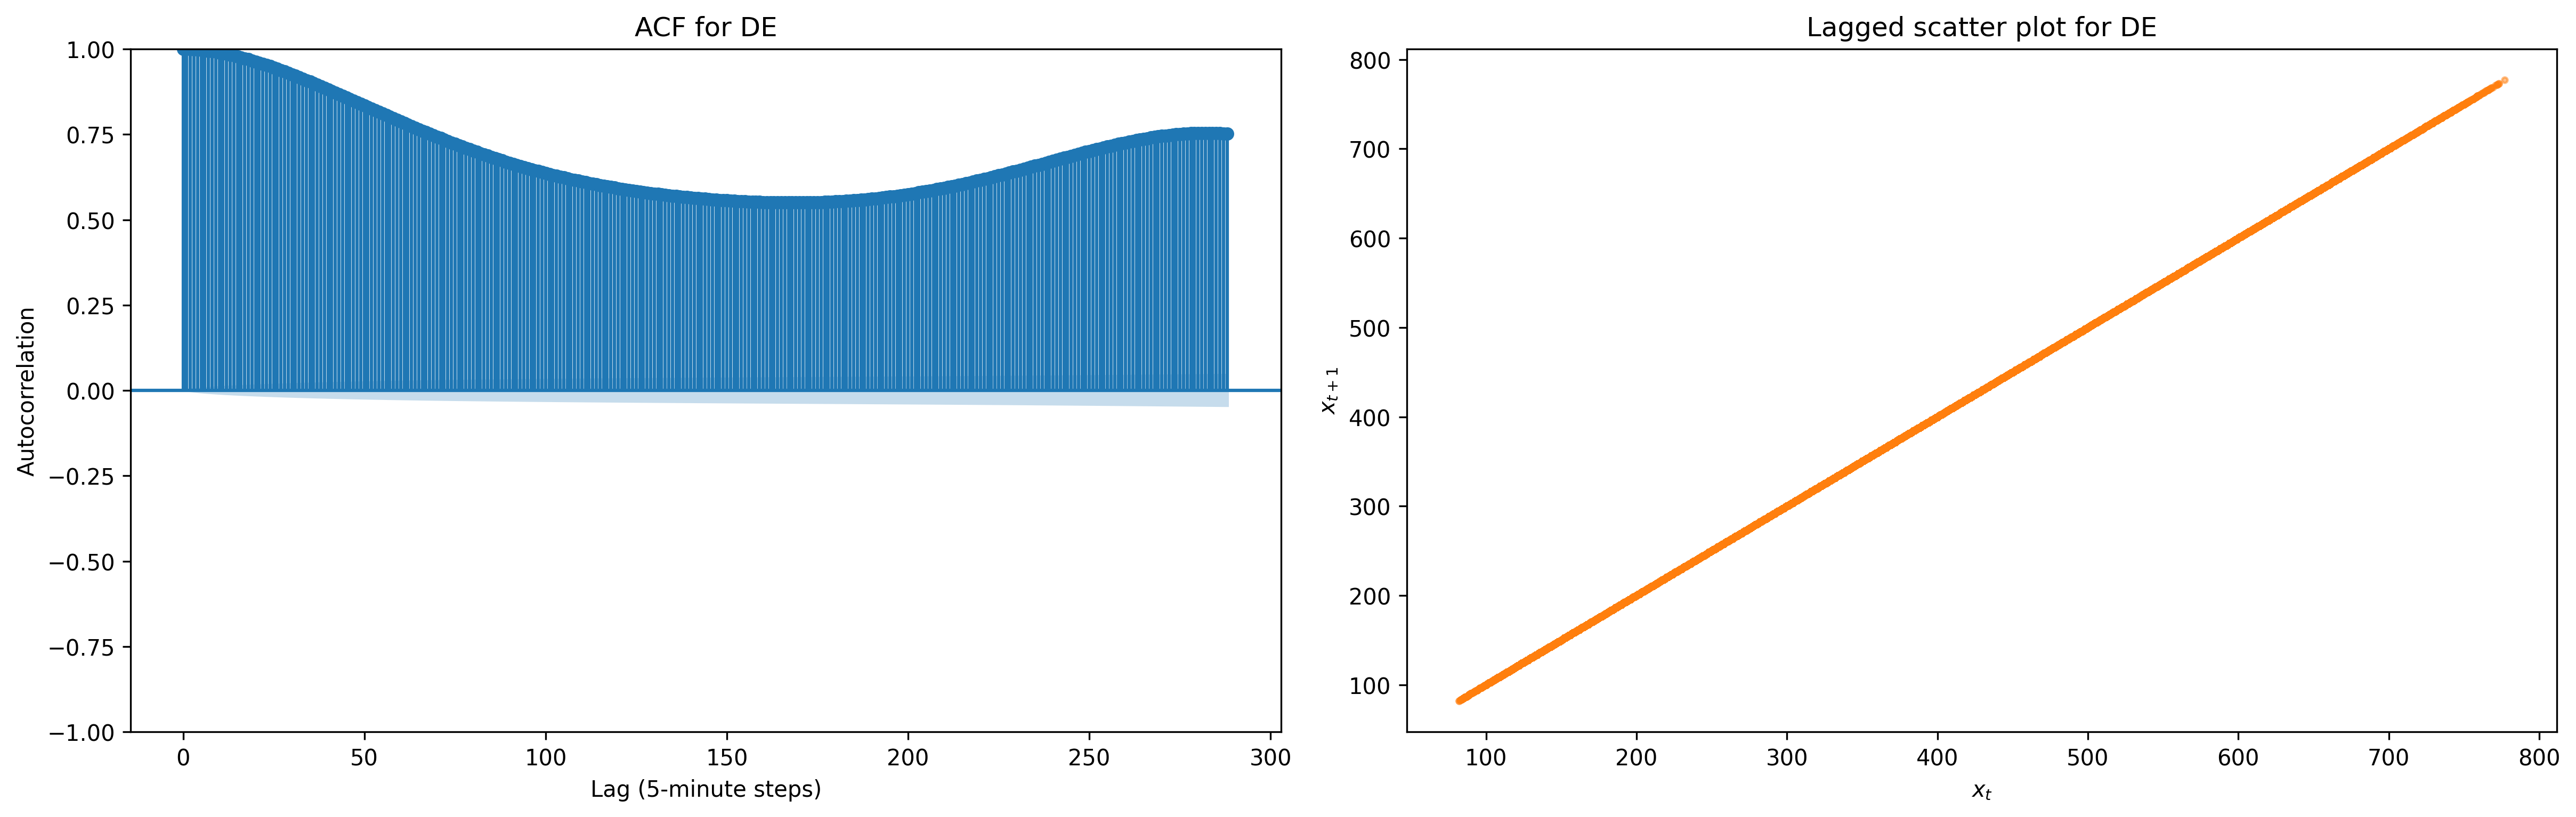
\includegraphics[width=\textwidth,height=0.58\textheight,keepaspectratio]{assets/acf_lag.png}

  \vspace{0.05cm}
  \begin{block}{Consequence for the training simulation}
    Lag-1 autocorrelation is 0.999 and the one-day lag is 0.694 for DE:
    chronological trace replay is more appropriate than IID sampling.
  \end{block}

\end{frame}

\begin{frame}[t]{Input Modeling}{Implications for our Simulation}

  \begin{enumerate}
    \item Use historical traces for evaluation, because temporal
      dependence is strong.
    \item Calibrate pause and resume thresholds per region, not globally.
    \item Compare policies on both CO$_2$ savings and wall-clock overhead.
    \item Treat clean regions differently: low baseline emissions
      reduce the benefit of aggressive pausing.
  \end{enumerate}

  \vspace{0.35cm}
  \begin{block}{Most important finding}
    Carbon-aware scheduling potential is driven by both the average grid mix
    \textbf{and} the temporal variability around that average.
  \end{block}

\end{frame}
